\chapter{Human-Agent Interaction Corpus}\label{sec.group.corpus}

% entry quote
\blockcquote[p. 156]{goffman1963}{By definition, an accessible engagement does not exhaust the situation; [\dots] What we find instead is some obligation and some effort on the part of both participants and bystanders to act as if the engagement were physically cut off from the rest of the situation.}

% introduction to the whole part with what is done in this chapter
%In the following three chapters I broaden the problem of \gls{addressee} recognition for \glspl{artificial agent} in two directions which become increasingly important when the agent is used over longer time periods and with changing interaction partners. 
%\blockquote{\Cref{hyp.fformation}: \hypfformation}
%On the other hand, when the \gls{robot} is in a \gls{conversational group} it needs to recognize its \gls{conversational role} to be able to act accordingly.
%This problem is stated in:
%\blockquote{\Cref{hyp.roles}: \hyproles}
To investigate \Cref{hyp.fformation}\rqnote{hyp.fformation}{\hypfformation} and \Cref{hyp.roles}\rqnote{hyp.roles}{\hyproles}, a corpus of open, multi-centric interactions between people and \glspl{artificial agent} is needed.
In this chapter, I discuss the requirements of such a corpus and present a suitable scenario.
On this basis, I create a corpus of interactions between a group of people and the \gls{flobi} agents in the \gls{csra}.
This corpus is utilized in the following chapters to examine the recognition of \glspl{conversational group} (\cref{ch.fformation}) and \glspl{conversational role} (\cref{ch.roles}) of \glspl{artificial agent}. 
 
\section{Introduction}

% 1. Opening context or background. 
As discussed in \cref{sec.rw.hi}, people who are \glsatt{copresence}, always interact with each other in some way.
In a \gls{focused interaction} they \gls{turn} towards each other, reduce their distance, and increase the frequency and duration of mutual gazes (\cref{sec.rw.hi.focused}).
Moreover, they can have different \glspl{conversational role} which are dynamically negotiated using the \gls{turn taking system}.
In an \gls{unfocused interaction}, people display that they are part of the situation.
They acknowledge the presence of others but direct their attention somewhere else to show \gls{civil inattention}.
They reduce mutual gazes, increase their distance and \gls{turn} away from each other (\cref{sec.rw.hi.unfocused}).
It is necessary for people to be able to distinguish and display whether and with whom they are in a focused or \gls{unfocused interaction}.
Otherwise, they are not able to act appropriately and may be perceived as offensive~\cite[p. 29, p. 157]{goffman1963}.

\Glspl{artificial agent}---e.g. in form of \glspl{robot} or \glspl{virtual agent}---are potential interaction partners.
In a \gls{smart environment} that contains interactive \glspl{artificial agent}, people are always in their \gls{copresence}.
%In contrast, a \glsatt{copresence} agent that is part of a \gls{focused interaction}, needs to adhere to the requirements of \glspl{focused interaction}.
%As presented in \cref{sec.rw.hi.focused} this includes maximizing mutual monitoring possibilities within the group and reducing the same from outside the group.
%Furthermore, it needs to mind its \gls{conversational role} and the dynamics of \gls{turn taking} (\cref{sec.rw.hi.focused}).
To be able to behave in a manner that is appropriate to the situation, an agent first needs to understand it.
As presented in \cref{sec.rw.hi.focused-rw.groups}, there already exists work on the detection of human-only \glspl{conversational group}.
However, work on the detection of mixed \glspl{conversational group} in \gls{hai} is sparse.
The possible effects of specific formations and the relevance of human \glspl{conversational group} for socially acceptable \glsatt{robot} navigation are more in focus of \gls{hai} research (\cref{sec.rw.hi.focused-rw.mixedgroups}).
As a sub-problem of \gls{conversational role} recognition, approaches to the recognition of utterances addressed towards the agent are presented in \cref{sec.rw.hi.focused-rw.addressing}.
However, the presented interactions are restricted.
The agent is controlled by a \gls{wizard}, its \gls{conversational group} is fixed or the participants are augmented with close-talk microphones.
To investigate, how dynamically changing \glspl{conversational group} with people and \glspl{artificial agent} can be detected and how the \glspl{conversational role} within such groups can be recognized, a fitting interaction corpus is required.
%In contrast, I investigate how \glspl{focused interaction} containing people and \glspl{artificial agent} can be recognized in a \gls{smart environment} and how this knowledge can further be applied to recognize the \gls{conversational role} of the agents.

% available corpora
In the \gls{conversational group} detection community there are multiple, frequently used datasets for the evaluation of recognition models.
The most widely adopted are \emph{Synthetic} and \emph{Coffee Break} from~\citewithauthor{Cristani2011}, \emph{IDIAP Poster Data} from~\citewithauthor{Hung2011}, \emph{Cocktail Party} form~\citewithauthor{Setti2013}, and \emph{GDet} from~\citewithauthor{Bazzani2013}.
They are used for the evaluation of vision based \gls{conversational group} detection models as performed by~\citewithauthor{Setti2015} and~\citewithauthor{Vascon2016}.
Furthermore, there are multi-modal datasets like \emph{SALSA} from~\citewithauthor{Alameda-Pineda2016} and \emph{MatchNMingle} from~\citewithauthor{Cabrera-Quiros2018}.
The authors use these datasets to evaluate multi-modal approaches to \gls{conversational group} detection and subsequent analyses of group properties.
All these datasets show similar situations:
A crowded place where people stand and interact at a poster presentation, coffee break, speed-dating or similar socializing event.
These scenarios are intentionally chosen to allow people to act as natural as possible while simultaneously allowing the observation of many interactions and changing groups.
None of these scenarios feature \glspl{artificial agent}.

Datasets for the analysis of \glspl{conversational role}, often use fixed groups of people without \glspl{artificial agent}~\cite{Jovanovic2006,Akhtiamov2017,Makino2018}.
If \glspl{artificial agent} are present in such interactions, they are controlled by a \gls{wizard}~\cite{VanTurnhout2005,Jayagopi2013a}, or only distinguish utterances addressed at them from others~\cite{Bohus2011,Skantze2014}.
Furthermore, these systems consider \glspl{conversational group} only as a distinction between interacting and non-interacting people, using simple heuristics.
%
Additionally, if people without experience in \gls{hai} find themselves in \gls{copresence} with an \gls{artificial agent} its novelty may lead to a higher amount of attention and overall amplified measures.
Therefore, a scenario is needed in which a group of people can freely interact with each other and with \glspl{artificial agent} for an extended time.
This way they can get accustomed to the situation and act more natural.

\section{Scenario}

To fulfil the presented requirements, I collect a new corpus in the \gls{csra}.
For a visualization of the recorded videos see \cref{fig:group-perspectives}.
\begin{figure}[htb]
  \centering
    \def\svgwidth{\textwidth}
    \input{generated/study-group-shots.pdf_tex}
    \caption[Group detection study video perspectives.]{\label{fig:group-perspectives} The 14 perspectives from which videos are recorded during the study. 
    The overview perspectives are in the top row (\emph{O}, blue background), 
    the web-cam perspectives are in the right column (\emph{W}, orange background), and the remaining images show top-down perspectives (\emph{T1:} kitchen and hallway with green background and \emph{T2:} living-room with violet background).
    }
\end{figure}
The corpus contains the following scenario:
A group is invited into the \gls{apartment} for a demonstration composed of three parts.
\begin{description}
    \item[Briefing] In the first part, the presenter---a person that is acquainted with the environment and realizes the demonstration---and the guests ga\-ther in front of the \gls{apartment}.
    The participants get an explanation about what the \gls{apartment} is, what is being recorded during the study, and their rights regarding data privacy.
    After the participants gave their consent, the main part of the demonstration begins.
    \item[Presentation] The presenter enters the \gls{apartment} together with the participants and guides them through the hallway, living room and kitchen.
    In each room the group stops and the presenter gives information about the \gls{apartment} or shows interaction possibilities.
    In the hallway and kitchen, respectively an interaction with the \gls{virtual agent} \gls{flobi}---the host of the \gls{apartment}---is performed.
    The living room is used to give information about the \gls{apartment}'s actuation and introspection capabilities.
    \item[Free Interaction] In the third part of the demonstration, the participants are allowed to freely chat, test the different control metaphors of the \gls{apartment} or interact with the \glspl{virtual agent}.
    During this period, the presenter remains in the \gls{apartment} to answer further questions.
\end{description}
The scenario is recorded using the \gls{apartment}'s study facilities.
The recording is started before the \gls{apartment} is entered and stopped after the last participant left.

\section{Recording}

With this approach I perform a long demonstration for a group of students and their lecturers.
The recording contains 
\begin{enumerate*}[label=(\arabic*)]
    \item four overview videos from the \gls{apartment}'s corners,
    \item two web-cam videos from the agents' perspective, 
    \item eight top-down videos,
    \item two audio streams, and 
    \item the communication between software components of the \gls{csra}.
To see the video perspectives, refer to \cref{fig:group-perspectives}.
\end{enumerate*}
This resulting \SI{57}{\minute} of unconstrained, mixed human and human-agent interaction are composed of \SI{20}{\minute} presentation and \SI{37}{\minute} free interaction. 
The participants are 8 women and 3 men---including the presenter.
This dataset is a good basis for the analysis of mixed, human-agent interactions.
Before it can be used to evaluate automatic \gls{conversational group} detection and \gls{conversational role} recognition in mixed human-agent interactions, some processing and annotation is required.
A visualisation of the annotations can be seen in \cref{fig:map-annotation}.
\begin{figure}[htb]
  \centering
    \def\svgwidth{\textwidth}
    \input{generated/csra_map_annotations.pdf_tex}
    \caption[Group and role annotations.]{\label{fig:map-annotation}
    Annotations of the scene from \cref{fig:group-perspectives}.
    The participant's and agent's poses are shown as triangles with annotated \emph{participant-id}.
    \Glspl{conversational group} are highlighted in yellow.
    \Glspl{conversational role} are shown in red (\gls{speaker}), green (\gls{addressee}), blue (\gls{side-participant}), and white (\gls{non-participant}).
    }
\end{figure}

\section{Annotation}

The study recording contains multiple video streams, audio streams and communication between software components of the \gls{csra}.
To be able to examine \cref{hyp.fformation,hyp.roles}, a set of ground truth annotations is required. 
A visualization of the annotations for the scene in \cref{fig:group-perspectives} can be seen in \cref{fig:map-annotation}.
To this end, the required information is annotated on the basis of the top-down videos of the hallway and kitchen \emph{T1}.
The remaining areas (\emph{T2}) of the \gls{apartment} are not annotated because they are not relevant for interactions with the \glspl{flobi}.
The following information is manually annotated:
\begin{enumerate*}[label=(\arabic*)]
    \item Pose (position and rotation) of all participants and \glspl{flobi},
    \item participant ids,
    \item all \glspl{conversational group} the \glspl{flobi} participate in, and
    \item \glspl{conversational role} for all annotated \glspl{conversational group}.
\end{enumerate*}
Annotations are done whenever a change in the participants pose, a group, or a role can be observed.
In comparison to annotating fixed time intervals, this reduces the amount of needed annotations and allows an arbitrary sampling of annotations.
Participants poses can be interpolated between annotations and groups and roles are static between changes.
Furthermore, poses of the same person, when annotated from multiple viewpoints, can be averaged to further enhance estimations of the participants pose.
The final dataset is created by sampling these annotations at a fixed rate of \SI{15}{\Hz}.
The overall distribution of group-sizes for the two agents at this sampling rate can be seen in \cref{fig:group-sizes}.
\begin{figure}[htb]
    \centering
    % Created by tikzDevice version 0.12
% !TEX encoding = UTF-8 Unicode
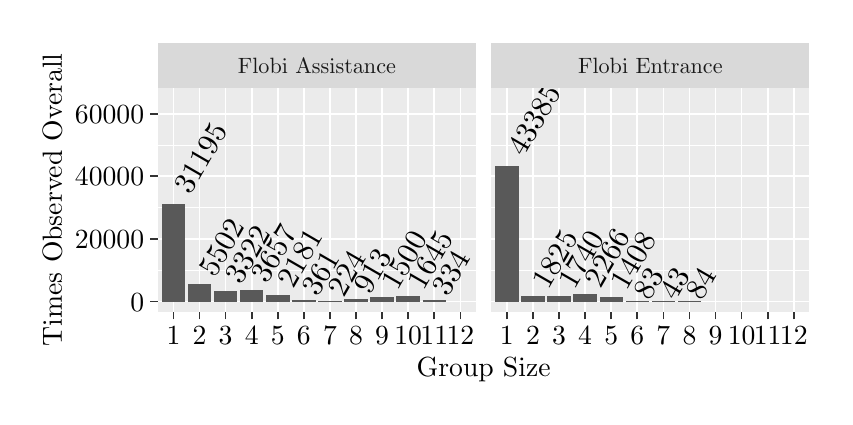
\begin{tikzpicture}[x=1pt,y=1pt]
\definecolor{fillColor}{RGB}{255,255,255}
\path[use as bounding box,fill=fillColor,fill opacity=0.00] (0,0) rectangle (288.00,133.49);
\begin{scope}
\path[clip] (  0.00,  0.00) rectangle (288.00,133.49);
\definecolor{drawColor}{RGB}{255,255,255}
\definecolor{fillColor}{RGB}{255,255,255}

\path[draw=drawColor,line width= 0.6pt,line join=round,line cap=round,fill=fillColor] (  0.00,  0.00) rectangle (288.00,133.49);
\end{scope}
\begin{scope}
\path[clip] ( 47.03, 30.86) rectangle (162.01,111.73);
\definecolor{fillColor}{gray}{0.92}

\path[fill=fillColor] ( 47.03, 30.86) rectangle (162.01,111.73);
\definecolor{drawColor}{RGB}{255,255,255}

\path[draw=drawColor,line width= 0.3pt,line join=round] ( 47.03, 45.85) --
	(162.01, 45.85);

\path[draw=drawColor,line width= 0.3pt,line join=round] ( 47.03, 68.47) --
	(162.01, 68.47);

\path[draw=drawColor,line width= 0.3pt,line join=round] ( 47.03, 91.09) --
	(162.01, 91.09);

\path[draw=drawColor,line width= 0.6pt,line join=round] ( 47.03, 34.54) --
	(162.01, 34.54);

\path[draw=drawColor,line width= 0.6pt,line join=round] ( 47.03, 57.16) --
	(162.01, 57.16);

\path[draw=drawColor,line width= 0.6pt,line join=round] ( 47.03, 79.78) --
	(162.01, 79.78);

\path[draw=drawColor,line width= 0.6pt,line join=round] ( 47.03,102.40) --
	(162.01,102.40);

\path[draw=drawColor,line width= 0.6pt,line join=round] ( 52.68, 30.86) --
	( 52.68,111.73);

\path[draw=drawColor,line width= 0.6pt,line join=round] ( 62.11, 30.86) --
	( 62.11,111.73);

\path[draw=drawColor,line width= 0.6pt,line join=round] ( 71.53, 30.86) --
	( 71.53,111.73);

\path[draw=drawColor,line width= 0.6pt,line join=round] ( 80.96, 30.86) --
	( 80.96,111.73);

\path[draw=drawColor,line width= 0.6pt,line join=round] ( 90.38, 30.86) --
	( 90.38,111.73);

\path[draw=drawColor,line width= 0.6pt,line join=round] ( 99.81, 30.86) --
	( 99.81,111.73);

\path[draw=drawColor,line width= 0.6pt,line join=round] (109.23, 30.86) --
	(109.23,111.73);

\path[draw=drawColor,line width= 0.6pt,line join=round] (118.66, 30.86) --
	(118.66,111.73);

\path[draw=drawColor,line width= 0.6pt,line join=round] (128.08, 30.86) --
	(128.08,111.73);

\path[draw=drawColor,line width= 0.6pt,line join=round] (137.51, 30.86) --
	(137.51,111.73);

\path[draw=drawColor,line width= 0.6pt,line join=round] (146.93, 30.86) --
	(146.93,111.73);

\path[draw=drawColor,line width= 0.6pt,line join=round] (156.36, 30.86) --
	(156.36,111.73);
\definecolor{fillColor}{gray}{0.35}

\path[fill=fillColor] ( 48.44, 34.54) rectangle ( 56.92, 69.82);

\path[fill=fillColor] ( 57.86, 34.54) rectangle ( 66.35, 40.76);

\path[fill=fillColor] ( 67.29, 34.54) rectangle ( 75.77, 38.30);

\path[fill=fillColor] ( 76.71, 34.54) rectangle ( 85.20, 38.67);

\path[fill=fillColor] ( 86.14, 34.54) rectangle ( 94.62, 37.01);

\path[fill=fillColor] ( 95.56, 34.54) rectangle (104.05, 34.95);

\path[fill=fillColor] (104.99, 34.54) rectangle (113.47, 34.79);

\path[fill=fillColor] (114.42, 34.54) rectangle (122.90, 35.57);

\path[fill=fillColor] (123.84, 34.54) rectangle (132.32, 36.23);

\path[fill=fillColor] (133.27, 34.54) rectangle (141.75, 36.40);

\path[fill=fillColor] (142.69, 34.54) rectangle (151.17, 34.92);
\definecolor{drawColor}{RGB}{0,0,0}

\node[text=drawColor,rotate= 60.00,anchor=base west,inner sep=0pt, outer sep=0pt, scale=  1.10] at ( 58.73, 72.70) {31195};

\node[text=drawColor,rotate= 60.00,anchor=base west,inner sep=0pt, outer sep=0pt, scale=  1.10] at ( 67.61, 42.68) {5502};

\node[text=drawColor,rotate= 60.00,anchor=base west,inner sep=0pt, outer sep=0pt, scale=  1.10] at ( 77.03, 40.22) {3322};

\node[text=drawColor,rotate= 60.00,anchor=base west,inner sep=0pt, outer sep=0pt, scale=  1.10] at ( 86.46, 40.60) {3657};

\node[text=drawColor,rotate= 60.00,anchor=base west,inner sep=0pt, outer sep=0pt, scale=  1.10] at ( 95.88, 38.93) {2181};

\node[text=drawColor,rotate= 60.00,anchor=base west,inner sep=0pt, outer sep=0pt, scale=  1.10] at (104.75, 35.91) {361};

\node[text=drawColor,rotate= 60.00,anchor=base west,inner sep=0pt, outer sep=0pt, scale=  1.10] at (114.18, 35.76) {224};

\node[text=drawColor,rotate= 60.00,anchor=base west,inner sep=0pt, outer sep=0pt, scale=  1.10] at (123.60, 36.54) {913};

\node[text=drawColor,rotate= 60.00,anchor=base west,inner sep=0pt, outer sep=0pt, scale=  1.10] at (133.58, 38.16) {1500};

\node[text=drawColor,rotate= 60.00,anchor=base west,inner sep=0pt, outer sep=0pt, scale=  1.10] at (143.01, 38.32) {1645};

\node[text=drawColor,rotate= 60.00,anchor=base west,inner sep=0pt, outer sep=0pt, scale=  1.10] at (151.88, 35.88) {334};
\end{scope}
\begin{scope}
\path[clip] (167.51, 30.86) rectangle (282.50,111.73);
\definecolor{fillColor}{gray}{0.92}

\path[fill=fillColor] (167.51, 30.86) rectangle (282.50,111.73);
\definecolor{drawColor}{RGB}{255,255,255}

\path[draw=drawColor,line width= 0.3pt,line join=round] (167.51, 45.85) --
	(282.50, 45.85);

\path[draw=drawColor,line width= 0.3pt,line join=round] (167.51, 68.47) --
	(282.50, 68.47);

\path[draw=drawColor,line width= 0.3pt,line join=round] (167.51, 91.09) --
	(282.50, 91.09);

\path[draw=drawColor,line width= 0.6pt,line join=round] (167.51, 34.54) --
	(282.50, 34.54);

\path[draw=drawColor,line width= 0.6pt,line join=round] (167.51, 57.16) --
	(282.50, 57.16);

\path[draw=drawColor,line width= 0.6pt,line join=round] (167.51, 79.78) --
	(282.50, 79.78);

\path[draw=drawColor,line width= 0.6pt,line join=round] (167.51,102.40) --
	(282.50,102.40);

\path[draw=drawColor,line width= 0.6pt,line join=round] (173.17, 30.86) --
	(173.17,111.73);

\path[draw=drawColor,line width= 0.6pt,line join=round] (182.59, 30.86) --
	(182.59,111.73);

\path[draw=drawColor,line width= 0.6pt,line join=round] (192.02, 30.86) --
	(192.02,111.73);

\path[draw=drawColor,line width= 0.6pt,line join=round] (201.44, 30.86) --
	(201.44,111.73);

\path[draw=drawColor,line width= 0.6pt,line join=round] (210.87, 30.86) --
	(210.87,111.73);

\path[draw=drawColor,line width= 0.6pt,line join=round] (220.29, 30.86) --
	(220.29,111.73);

\path[draw=drawColor,line width= 0.6pt,line join=round] (229.72, 30.86) --
	(229.72,111.73);

\path[draw=drawColor,line width= 0.6pt,line join=round] (239.14, 30.86) --
	(239.14,111.73);

\path[draw=drawColor,line width= 0.6pt,line join=round] (248.57, 30.86) --
	(248.57,111.73);

\path[draw=drawColor,line width= 0.6pt,line join=round] (257.99, 30.86) --
	(257.99,111.73);

\path[draw=drawColor,line width= 0.6pt,line join=round] (267.42, 30.86) --
	(267.42,111.73);

\path[draw=drawColor,line width= 0.6pt,line join=round] (276.84, 30.86) --
	(276.84,111.73);
\definecolor{fillColor}{gray}{0.35}

\path[fill=fillColor] (168.93, 34.54) rectangle (177.41, 83.61);

\path[fill=fillColor] (178.35, 34.54) rectangle (186.83, 36.60);

\path[fill=fillColor] (187.78, 34.54) rectangle (196.26, 36.51);

\path[fill=fillColor] (197.20, 34.54) rectangle (205.68, 37.10);

\path[fill=fillColor] (206.63, 34.54) rectangle (215.11, 36.13);

\path[fill=fillColor] (216.05, 34.54) rectangle (224.54, 34.63);

\path[fill=fillColor] (225.48, 34.54) rectangle (233.96, 34.59);

\path[fill=fillColor] (234.90, 34.54) rectangle (243.39, 34.63);
\definecolor{drawColor}{RGB}{0,0,0}

\node[text=drawColor,rotate= 60.00,anchor=base west,inner sep=0pt, outer sep=0pt, scale=  1.10] at (179.22, 86.49) {43385};

\node[text=drawColor,rotate= 60.00,anchor=base west,inner sep=0pt, outer sep=0pt, scale=  1.10] at (188.09, 38.53) {1825};

\node[text=drawColor,rotate= 60.00,anchor=base west,inner sep=0pt, outer sep=0pt, scale=  1.10] at (197.52, 38.43) {1740};

\node[text=drawColor,rotate= 60.00,anchor=base west,inner sep=0pt, outer sep=0pt, scale=  1.10] at (206.94, 39.02) {2266};

\node[text=drawColor,rotate= 60.00,anchor=base west,inner sep=0pt, outer sep=0pt, scale=  1.10] at (216.37, 38.05) {1408};

\node[text=drawColor,rotate= 60.00,anchor=base west,inner sep=0pt, outer sep=0pt, scale=  1.10] at (224.69, 34.64) {83};

\node[text=drawColor,rotate= 60.00,anchor=base west,inner sep=0pt, outer sep=0pt, scale=  1.10] at (234.12, 34.60) {43};

\node[text=drawColor,rotate= 60.00,anchor=base west,inner sep=0pt, outer sep=0pt, scale=  1.10] at (243.54, 34.64) {84};
\end{scope}
\begin{scope}
\path[clip] ( 47.03,111.73) rectangle (162.01,127.99);
\definecolor{fillColor}{gray}{0.85}

\path[fill=fillColor] ( 47.03,111.73) rectangle (162.01,127.99);
\definecolor{drawColor}{gray}{0.10}

\node[text=drawColor,anchor=base,inner sep=0pt, outer sep=0pt, scale=  0.80] at (104.52,117.11) {Flobi Assistance};
\end{scope}
\begin{scope}
\path[clip] (167.51,111.73) rectangle (282.50,127.99);
\definecolor{fillColor}{gray}{0.85}

\path[fill=fillColor] (167.51,111.73) rectangle (282.50,127.99);
\definecolor{drawColor}{gray}{0.10}

\node[text=drawColor,anchor=base,inner sep=0pt, outer sep=0pt, scale=  0.80] at (225.01,117.11) {Flobi Entrance};
\end{scope}
\begin{scope}
\path[clip] (  0.00,  0.00) rectangle (288.00,133.49);
\definecolor{drawColor}{gray}{0.20}

\path[draw=drawColor,line width= 0.6pt,line join=round] ( 52.68, 28.11) --
	( 52.68, 30.86);

\path[draw=drawColor,line width= 0.6pt,line join=round] ( 62.11, 28.11) --
	( 62.11, 30.86);

\path[draw=drawColor,line width= 0.6pt,line join=round] ( 71.53, 28.11) --
	( 71.53, 30.86);

\path[draw=drawColor,line width= 0.6pt,line join=round] ( 80.96, 28.11) --
	( 80.96, 30.86);

\path[draw=drawColor,line width= 0.6pt,line join=round] ( 90.38, 28.11) --
	( 90.38, 30.86);

\path[draw=drawColor,line width= 0.6pt,line join=round] ( 99.81, 28.11) --
	( 99.81, 30.86);

\path[draw=drawColor,line width= 0.6pt,line join=round] (109.23, 28.11) --
	(109.23, 30.86);

\path[draw=drawColor,line width= 0.6pt,line join=round] (118.66, 28.11) --
	(118.66, 30.86);

\path[draw=drawColor,line width= 0.6pt,line join=round] (128.08, 28.11) --
	(128.08, 30.86);

\path[draw=drawColor,line width= 0.6pt,line join=round] (137.51, 28.11) --
	(137.51, 30.86);

\path[draw=drawColor,line width= 0.6pt,line join=round] (146.93, 28.11) --
	(146.93, 30.86);

\path[draw=drawColor,line width= 0.6pt,line join=round] (156.36, 28.11) --
	(156.36, 30.86);
\end{scope}
\begin{scope}
\path[clip] (  0.00,  0.00) rectangle (288.00,133.49);
\definecolor{drawColor}{RGB}{0,0,0}

\node[text=drawColor,anchor=base,inner sep=0pt, outer sep=0pt, scale=  1.00] at ( 52.68, 19.03) { 1};

\node[text=drawColor,anchor=base,inner sep=0pt, outer sep=0pt, scale=  1.00] at ( 62.11, 19.03) { 2};

\node[text=drawColor,anchor=base,inner sep=0pt, outer sep=0pt, scale=  1.00] at ( 71.53, 19.03) { 3};

\node[text=drawColor,anchor=base,inner sep=0pt, outer sep=0pt, scale=  1.00] at ( 80.96, 19.03) { 4};

\node[text=drawColor,anchor=base,inner sep=0pt, outer sep=0pt, scale=  1.00] at ( 90.38, 19.03) { 5};

\node[text=drawColor,anchor=base,inner sep=0pt, outer sep=0pt, scale=  1.00] at ( 99.81, 19.03) { 6};

\node[text=drawColor,anchor=base,inner sep=0pt, outer sep=0pt, scale=  1.00] at (109.23, 19.03) { 7};

\node[text=drawColor,anchor=base,inner sep=0pt, outer sep=0pt, scale=  1.00] at (118.66, 19.03) { 8};

\node[text=drawColor,anchor=base,inner sep=0pt, outer sep=0pt, scale=  1.00] at (128.08, 19.03) { 9};

\node[text=drawColor,anchor=base,inner sep=0pt, outer sep=0pt, scale=  1.00] at (137.51, 19.03) {10};

\node[text=drawColor,anchor=base,inner sep=0pt, outer sep=0pt, scale=  1.00] at (146.93, 19.03) {11};

\node[text=drawColor,anchor=base,inner sep=0pt, outer sep=0pt, scale=  1.00] at (156.36, 19.03) {12};
\end{scope}
\begin{scope}
\path[clip] (  0.00,  0.00) rectangle (288.00,133.49);
\definecolor{drawColor}{gray}{0.20}

\path[draw=drawColor,line width= 0.6pt,line join=round] (173.17, 28.11) --
	(173.17, 30.86);

\path[draw=drawColor,line width= 0.6pt,line join=round] (182.59, 28.11) --
	(182.59, 30.86);

\path[draw=drawColor,line width= 0.6pt,line join=round] (192.02, 28.11) --
	(192.02, 30.86);

\path[draw=drawColor,line width= 0.6pt,line join=round] (201.44, 28.11) --
	(201.44, 30.86);

\path[draw=drawColor,line width= 0.6pt,line join=round] (210.87, 28.11) --
	(210.87, 30.86);

\path[draw=drawColor,line width= 0.6pt,line join=round] (220.29, 28.11) --
	(220.29, 30.86);

\path[draw=drawColor,line width= 0.6pt,line join=round] (229.72, 28.11) --
	(229.72, 30.86);

\path[draw=drawColor,line width= 0.6pt,line join=round] (239.14, 28.11) --
	(239.14, 30.86);

\path[draw=drawColor,line width= 0.6pt,line join=round] (248.57, 28.11) --
	(248.57, 30.86);

\path[draw=drawColor,line width= 0.6pt,line join=round] (257.99, 28.11) --
	(257.99, 30.86);

\path[draw=drawColor,line width= 0.6pt,line join=round] (267.42, 28.11) --
	(267.42, 30.86);

\path[draw=drawColor,line width= 0.6pt,line join=round] (276.84, 28.11) --
	(276.84, 30.86);
\end{scope}
\begin{scope}
\path[clip] (  0.00,  0.00) rectangle (288.00,133.49);
\definecolor{drawColor}{RGB}{0,0,0}

\node[text=drawColor,anchor=base,inner sep=0pt, outer sep=0pt, scale=  1.00] at (173.17, 19.03) { 1};

\node[text=drawColor,anchor=base,inner sep=0pt, outer sep=0pt, scale=  1.00] at (182.59, 19.03) { 2};

\node[text=drawColor,anchor=base,inner sep=0pt, outer sep=0pt, scale=  1.00] at (192.02, 19.03) { 3};

\node[text=drawColor,anchor=base,inner sep=0pt, outer sep=0pt, scale=  1.00] at (201.44, 19.03) { 4};

\node[text=drawColor,anchor=base,inner sep=0pt, outer sep=0pt, scale=  1.00] at (210.87, 19.03) { 5};

\node[text=drawColor,anchor=base,inner sep=0pt, outer sep=0pt, scale=  1.00] at (220.29, 19.03) { 6};

\node[text=drawColor,anchor=base,inner sep=0pt, outer sep=0pt, scale=  1.00] at (229.72, 19.03) { 7};

\node[text=drawColor,anchor=base,inner sep=0pt, outer sep=0pt, scale=  1.00] at (239.14, 19.03) { 8};

\node[text=drawColor,anchor=base,inner sep=0pt, outer sep=0pt, scale=  1.00] at (248.57, 19.03) { 9};

\node[text=drawColor,anchor=base,inner sep=0pt, outer sep=0pt, scale=  1.00] at (257.99, 19.03) {10};

\node[text=drawColor,anchor=base,inner sep=0pt, outer sep=0pt, scale=  1.00] at (267.42, 19.03) {11};

\node[text=drawColor,anchor=base,inner sep=0pt, outer sep=0pt, scale=  1.00] at (276.84, 19.03) {12};
\end{scope}
\begin{scope}
\path[clip] (  0.00,  0.00) rectangle (288.00,133.49);
\definecolor{drawColor}{RGB}{0,0,0}

\node[text=drawColor,anchor=base east,inner sep=0pt, outer sep=0pt, scale=  1.00] at ( 42.08, 31.09) {0};

\node[text=drawColor,anchor=base east,inner sep=0pt, outer sep=0pt, scale=  1.00] at ( 42.08, 53.72) {20000};

\node[text=drawColor,anchor=base east,inner sep=0pt, outer sep=0pt, scale=  1.00] at ( 42.08, 76.34) {40000};

\node[text=drawColor,anchor=base east,inner sep=0pt, outer sep=0pt, scale=  1.00] at ( 42.08, 98.96) {60000};
\end{scope}
\begin{scope}
\path[clip] (  0.00,  0.00) rectangle (288.00,133.49);
\definecolor{drawColor}{gray}{0.20}

\path[draw=drawColor,line width= 0.6pt,line join=round] ( 44.28, 34.54) --
	( 47.03, 34.54);

\path[draw=drawColor,line width= 0.6pt,line join=round] ( 44.28, 57.16) --
	( 47.03, 57.16);

\path[draw=drawColor,line width= 0.6pt,line join=round] ( 44.28, 79.78) --
	( 47.03, 79.78);

\path[draw=drawColor,line width= 0.6pt,line join=round] ( 44.28,102.40) --
	( 47.03,102.40);
\end{scope}
\begin{scope}
\path[clip] (  0.00,  0.00) rectangle (288.00,133.49);
\definecolor{drawColor}{RGB}{0,0,0}

\node[text=drawColor,anchor=base,inner sep=0pt, outer sep=0pt, scale=  1.00] at (164.76,  7.44) {Group Size};
\end{scope}
\begin{scope}
\path[clip] (  0.00,  0.00) rectangle (288.00,133.49);
\definecolor{drawColor}{RGB}{0,0,0}

\node[text=drawColor,rotate= 90.00,anchor=base,inner sep=0pt, outer sep=0pt, scale=  1.00] at ( 12.39, 71.30) {Times Observed Overall};
\end{scope}
\end{tikzpicture}

    \caption[Distribution of group sizes of agents.]{\label{fig:group-sizes}
    The distribution of observed group sizes for the two agents in the group annotations of the corpus.
    The counts are additionally shown on top of the bars.
    A group size of 1 means that the agent is alone---not in a group with others.
    }
\end{figure}

\section{Automatic Data Extraction}\label{sec.group.extraction}

To assess the possibilities of fully automatic recognition of \glspl{conversational group} and \glspl{conversational role}, the following features are extracted from the system communication recordings:
\begin{enumerate*}[label=(\arabic*)]
   \item Positions of persons in the \gls{apartment} (at \SI{30}{\Hz}) from the person tracking system. Furthermore, in the \gls{fov} of both \glspl{flobi} (\(W\) perspectives in \cref{fig:group-perspectives}): 
   \item the \gls{roi} of each detected face,
   \item the recognized gaze-directions, and
   \item the detected facial landmarks (A visualization of these features can be seen in \vref{fig:meka-features}). Finally, for each agent
   \item whether it is speaking.
\end{enumerate*}

As the person tracking of the \gls{csra} does not provide rotational information, I additionally apply the~\citesoftware{openposegit} to the overview recordings (\emph{O} in \cref{fig:group-perspectives}) to detect 2D key-points of participants in video coordinates (see \cref{fig:group-openpose}).
\begin{figure}[htb]
    \centering
    \def\svgwidth{0.95\textwidth}
    \begin{footnotesize}
    \input{generated/study-group-shots-openpose.pdf_tex}
    \end{footnotesize}
    \caption[Automatic pose extraction.]{\label{fig:group-openpose}
    Visualization of the automatic pose extraction.
    The image shows the scene in \cref{fig:group-perspectives}, from the perspective of \(C_3\) (see \cref{fig:map-annotation}), augmented with person key-points as they are detected by~\citewithauthor{openposegit}.
    White circles (\(A\), \(C\), \(E\), \(G\), \(H\), and the \emph{false-positive} \(I\)) depict positions as they were detected by the \gls{apartment}'s person tracking system.
    Red arrows (\(B\), \(C\), \(D\), \(E\), and \(F\)) depict poses---position and rotation---as they were derived from the results of~\citewithauthor{openposegit}.
    The information used to derive poses is highlighted for \(F\).
    In this case, violet points depict points of the feet that are used to calculate the position (green point), gray arrows show rejected orientation hypotheses, and the yellow arrow depicts which orientation hypothesis was accepted.
    }
\end{figure}
On the basis of these key-points I create additional person hypotheses as follows:
For each detected person, the mean of all detected feet-key-points is calculated as the position in image coordinates.
The person's orientation is estimated from the following orientation-candidate vectors:
\begin{description}
    \item[shoulders] perpendicular to \(\text{left shoulder} \rightarrow \text{right shoulder}\)
    \item[hip] perpendicular to \(\text{left hip} \rightarrow \text{right hip}\)
    \item[left foot] along \(\text{left heel} \rightarrow \text{left big toe}\)
    \item[right foot] along \(\text{right heel} \rightarrow \text{right big toe}\)
\end{description}
The longest of these vectors is chosen as the most reliable cue and its direction accepted as the person's orientation in image coordinates.
Transforming this position and orientation into the floor-plane of the \gls{apartment}, results in an additional source for automatic tracking of persons in the \gls{apartment}.

To fuse detections from multiple camera perspectives and the person tracking, and select the corresponding annotations, the optimal assignment is calculated using the ~\citesoftware{hungarian}.
This identification of person percepts allows the evaluation of the fully automatic detections.
A visualization of the annotated and detected overall movements of the participants in the corpus can be seen in \cref{fig:group-person-movement}.
\begin{figure}[htb]
    \centering
    \def\svgwidth{1.0\textwidth}
    \input{generated/ffm-movements.pdf_tex}
    \caption[Movements in annotation and detection.]{\label{fig:group-person-movement}
    All positions of participants and agents in the \emph{T1}-region during the study.
    Observations are sampled at \SI{15}{\Hz} from the annotations (left) and automatic detections (right).
    Automatic detections are created by fusing results of the \gls{apartment}'s person tracking and the person detection based on \citewithauthor{openposegit} keypoint detection.
    Each side shows \(\approx7\cdot10^5\) observations as points with 95\% transparency.
    Different colours represent the positions of different persons.
    \Gls{flobi} positions are constant.
    }
\end{figure}

The annotated and automatically extracted poses and annotations of \glspl{conversational group} can be used to examine \Cref{hyp.fformation}\rqnote{hyp.fformation}{\hypfformation}.
The results of the \gls{apartment}'s face detection and gaze recognition can be used for further analyses.
Furthermore, \Cref{hyp.roles}\rqnote{hyp.roles}{\hyproles} can be investigated by combining the results of the \gls{conversational group} detection with other features.
These investigations are performed in \cref{ch.fformation,ch.roles}.

\section{Summary}\label{sec.group.corpus.summary}

In this chapter I created the foundation for the investigation of \Cref{hyp.fformation}\rqnote{hyp.fformation}{\hypfformation} and \Cref{hyp.roles}\rqnote{hyp.roles}{\hyproles}.
To this end, I presented the requirements a corpus for the investigation of \glspl{conversational group} and \glspl{conversational role} in dynamically changing interactions of humans with \glspl{artificial agent} needs to meet.
After showing that available corpora do not meet the requirements, I presented a new \gls{hai} scenario in the \gls{csra}.
I recorded an extended interaction and created an approach for fully automatic detection of person positions and orientations.
Finally, I created ground truth annotations of \glspl{conversational group} and \glspl{conversational role}, which can be used for the investigation of the presented research questions. 
